\documentclass[12pt,a4paper]{article}
\usepackage{amsmath,amscd,amsbsy,amssymb,latexsym,url,bm,amsthm}
\usepackage{epsfig,graphicx,subfigure}
\usepackage{enumitem,balance}
\usepackage{wrapfig}
\usepackage{mathrsfs,euscript}
\usepackage[usenames]{xcolor}
\usepackage{hyperref}
\usepackage[vlined,ruled,linesnumbered]{algorithm2e}
\hypersetup{colorlinks=true,linkcolor=black}

\newtheorem{theorem}{Theorem}
\newtheorem{lemma}[theorem]{Lemma}
\newtheorem{proposition}[theorem]{Proposition}
\newtheorem{corollary}[theorem]{Corollary}
\newtheorem{exercise}{Exercise}
\newtheorem*{solution}{Solution}
\newtheorem{definition}{Definition}
\theoremstyle{definition}

\renewcommand{\thefootnote}{\fnsymbol{footnote}}

\newcommand{\postscript}[2]
 {\setlength{\epsfxsize}{#2\hsize}
  \centerline{\epsfbox{#1}}}

\renewcommand{\baselinestretch}{1.0}

\setlength{\oddsidemargin}{-0.365in}
\setlength{\evensidemargin}{-0.365in}
\setlength{\topmargin}{-0.3in}
\setlength{\headheight}{0in}
\setlength{\headsep}{0in}
\setlength{\textheight}{10.1in}
\setlength{\textwidth}{7in}
\makeatletter \renewenvironment{proof}[1][Proof] {\par\pushQED{\qed}\normalfont\topsep6\p@\@plus6\p@\relax\trivlist\item[\hskip\labelsep\bfseries#1\@addpunct{.}]\ignorespaces}{\popQED\endtrivlist\@endpefalse} \makeatother
\makeatletter
\renewenvironment{solution}[1][Solution] {\par\pushQED{\qed}\normalfont\topsep6\p@\@plus6\p@\relax\trivlist\item[\hskip\labelsep\bfseries#1\@addpunct{.}]\ignorespaces}{\popQED\endtrivlist\@endpefalse} \makeatother

\begin{document}
\noindent

%========================================================================
\noindent\framebox[\linewidth]{\shortstack[c]{
\Large{\textbf{Lab07-Network Flow}}\vspace{1mm}\\
CS214-Algorithm and Complexity, Xiaofeng Gao, Spring 2019.}}


\begin{center}
\footnotesize{\color{red}$*$ If there is any problem, please contact TA Mingran Peng.}\par
% Please write down your name, student id and email.
\footnotesize{\color{blue}$*$ Name:KylinChen  \quad Student ID:517030910155 \quad Email:k1017856853@icloud.com }
\end{center}
\begin{enumerate}
    
    \item
    Remember the network problems in last lab?\par
    Consider there is a network consists $n$ computers. For some pairs of computers, a wire $i$ exists in the pair, which means these two computers can communicate with delay $t_i$.\par
The distance of two computers are defined as their communication delay. Design an algorithm to compute the maximum distance in the network.\par
You need to provide the pseudo code and analyze the time complexity.\par

\begin{solution}\item
\renewcommand{\qedsymbol}{}


    For this Problem, we give two algorithm:

    \textbf{(1) Modified\ Floyd-Warshall\ Algorithm: }Now that we want to compare path distance in the graph, we can use Floyd-Warshall Algorithm to calculate the all-pair minimun path in the graph. Finally we can use brute-force to find the maximum one in all the shortest distance-pairs.

    \begin{minipage}[t]{0.9\textwidth}
        \begin{algorithm}[H]
            \KwIn{$C_{i,j}$ ; $n$;}
            %\BlankLine
            \caption{$Modified\ Floyd-Warshall\ Algorithm$}
            \label{ALG1}
            $Res\leftarrow 0$\;
            \For{$i\leftarrow 1$ \textbf{to} $n$}{
                \For{$j\leftarrow 1$ \textbf{to} $n$}{
                    \If{$C_{i,j}$ exists}{
                        $Dis[i][j] \leftarrow C_{i,j}$\;
                    }
                    \Else{
                        $Dis[i][j] \leftarrow \infty$\;
                    }
                }
            }
            \For{$k\leftarrow 1$ \textbf{to} $n$}{
                \For{$i\leftarrow 1$ \textbf{to} $n$}{
                    \For{$j\leftarrow 1$ \textbf{to} $n$}{
                        \If{$Dis[i][j] > Dis[i][k] +Dis[k][j]$}{
                            $Dis[i][j] = Dis[i][k] +Dis[k][j]$\;
                        }
                    }
                }
            }
            \For{$i\leftarrow 1$ \textbf{to} $n$}{
                \For{$j\leftarrow 1$ \textbf{to} $n$}{
                    \If{$Dis[i][j] > Res$}{
                            $Res = Dis[i][j]$\;
                        }
                }
            }
            $return\ Res $\;
        \end{algorithm}
        \end{minipage}
        \hfill
    \item 
    In Algorithm.\ref{ALG1}, we use three-nesting-loop to find the symmetrically maximun distance, every loop execute $n$ times. Then we use extra 2-loops of n steps to find the maximal distance. It means this algorithm runs in $\Theta(n^3+n^2)=O(n^3)$ time.\item

    
    \textbf{(2) Modified\ Bellman-Ford Algorithm: }As Algorithm.\ref{ALG1}, once we want to find the maximum shortest-path between all the reachable node-pairs, we can use Bellman-Ford Algorithm to calculate all the single-source shortest distance one by one. In the calculating process, we use a variable $Res$ to maintain the maximum.
    
    \begin{minipage}[t]{0.9\textwidth}
        \begin{algorithm}[H]
            \KwIn{node number $n$;}
            \KwOut{$Res$ as maximum path length}
            %\BlankLine
            \caption{Modified\ Bellman-Ford\ Algorithm}
            \label{ALG2}
            \BlankLine
            $Res\leftarrow 0$\;
            \For{$j\leftarrow 1$ \textbf{to} $n$}{
                \For{$node\ u \in V$}{
                    $M[0,u] \leftarrow \infty$\;
                }
                $M[0,j] \leftarrow 0$\;
                \For{$i\leftarrow 1$ \textbf{to} $n-1$}{
                    \For{$node\ v \in V$}{
                        \If{$M[v]$ has been updated in previous iteration}{
                            \For{$edge(u, v) \in E$}{
                                $M[i, u] \leftarrow min\{M[i - 1, u], M[i - 1, v] + w(u, v)\}$\;
                                
                            }
                        }
                    }
                }
                \For{$node\ v \in V$}{
                    \If{$Res<M[v]$}{
                        $Res=M[v]$\;
                    }
                }
            }
            $return\ Res $\;
       \end{algorithm}
       \end{minipage}
       \hfill

       \item In Algorithm.\ref{ALG2}, we use m-loop to set every point as the source point, every loop execute Modified Bellman-Ford Algorithm and a |V|-step comparasion, it means this algorithm runs in $O((V\cdot E+V)\times V)=O(V^2\cdot E)$ time.

\end{solution}

\item
   Suppose you are traveling through a country defined as a directed graph $G=(V,E)$. You start from vertex $s$ and want to go to $e$. For each $i\in E$, there is a $w_i$ regarding the cost for traveling via $i$. Some times $w_i<0$ which means you can earn money by traveling.(Do not ask why.) Here you need to design an algorithm satisfying the following demands:\par
   \begin{enumerate}
   \item Find the minimum cost from $s$ to $e$. The problem guarantee that there is a path from $s$ to $e$.\par
   \item Indicate whether there is a circle in $G$, that by traveling through this circle you can earn money continually.\par
   \end{enumerate}
   You need to provide the pseudo code and analyze the time complexity.\par

\begin{solution}\item
\renewcommand{\qedsymbol}{}
\begin{itemize}
\item [(a)] Now that we want to find the minimum-cost path between two fixed point, we can use Bellman-Ford Algorithm to solve it. Moreover, once there exists a negative cycle, we can decrease our cost(by earning money), which means minimum doesn't exists. Therefore, we should add a constrain that we don't pass each edge twice.

\begin{minipage}[t]{0.8\textwidth}
        \begin{algorithm}[H]
            \KwIn{node number $n$ ; edge wight $w_{i,j}$ ; $s$ ; $t$ ;}
            \KwOut{$Res$ as maximum distance from $s$ to $e$;}
            %\BlankLine
            \caption{Bellman-Ford\ Algorithm}
            \label{ALG3}
            \BlankLine
            $Res\leftarrow 0$\;
            
                \For{$node\ u \in V$}{
                    $M[0,u] \leftarrow \infty$\;
                }
                $M[0,t] \leftarrow 0$\;
                \For{$i\leftarrow 1$ \textbf{to} $n-1$}{
                    \For{$node\ v \in V$}{
                        \If{$M[v]$ has been updated in previous iteration}{
                            \For{$edge(u, v) \in E$}{
                                $M[i, u] \leftarrow min\{M[i - 1, u], M[i - 1, v] + w(u, v)\}$\;
                                
                            }
                        }
                    }
                }

            $return\ M[n-1,s] $\;
       \end{algorithm}
       \end{minipage}
       \hfill
       \par 
       In Algorithm.\ref{ALG3}, we use a three-nesting-loop to achieve. The outer layer loop $|V|$ times while inner layer loop $|E|$ times, it means this algorithm runs in $O(VE)$ time.

\item [(b)] In the Bellman-Ford Algorithm, we can calculate the $M[n,u]$ for $u$ in $V$, once $M[n,u] < M[n-1,u]$, there must exist a negative cycle because the longest path in a $n-nodes$ graph contains $n-1$ edges.

\begin{minipage}[t]{0.8\textwidth}
        \begin{algorithm}[H]
            \KwIn{node number $n$ ; edge wight $w_{i,j}$ ; $s$ ; $t$ ;}
            \KwOut{$True$ means there exists negative cycle, $False$ oppesites;}
            %\BlankLine
            \caption{Bellman-Ford\ Algorithm}
            \label{ALG4}
            \BlankLine
            $Res\leftarrow 0$\;
            
                \For{$node\ u \in V$}{
                    $M[0,u] \leftarrow \infty$\;
                }
                $M[0,t] \leftarrow 0$\;
                \For{$i\leftarrow 1$ \textbf{to} $n-1$}{
                    \For{$node\ v \in V$}{
                        \If{$M[v]$ has been updated in previous iteration}{
                            \For{$edge(u, v) \in E$}{
                                $M[i, u] \leftarrow min\{M[i - 1, u], M[i - 1, v] + w(u, v)\}$\;
                                
                            }
                        }
                    }
                }
                \For{$node\ v \in V$}{
                        \If{$M[v]$ has been updated in previous iteration}{
                            \For{$edge(u, v) \in E$}{
                                \If{$M[n-1, u]>M[n-1, v] + w(u, v)$}{
                                    $return\ $True$ $\;
                                }
                            }
                        }
                    }

            $return\ $False$ $\;
       \end{algorithm}
       \end{minipage}
       \hfill
       \par 
       In Algorithm.\ref{ALG4}, we use Bellman-Ford Algorithm to detect the existence of negative cycle, and the extra steps only cost $|V|$ time, which is less than the major manufacture of Bellman-Ford Algorithm. Therefore Algorithm.\ref{ALG4} runs in $O(VE)$ time.

\end{itemize}
\end{solution}

\item

\color{red}(Bonus)\color{black}
Suppose you are a staff of SJTU who is in charge of arranging lessons. Suppose you have $n$ time slots, $n$ lessons and $n$ professors. Clearly, you should assign exactly one time slot and one lesson to every professor. A lesson or a time slot should be assigned to exactly one professor. \par
For each professor, he will prefer some certain time slots among these $n$ time slots, and prefer to taught some certain lessons among these $n$ lessons.\par
A professor will be satisfied iff you arrange him both his preferred lesson and preferred time slot. Your goal is to satisfy as many professors as you can. Design an algorithm to output how many professors can you satisfy at most.\par 
Notice that this problem is really hard, even draft idea is welcomed.\par
(Hint: Treat time slots, lessons, professors as nodes. Construct edges according to professors' preference. Use network flow algorithm to solve it. )

\begin{solution}\item
\renewcommand{\qedsymbol}{}
For this problem, we can use a Network-Flow model to solve this problem.\item
\begin{itemize}
\item [(1)]\textbf{Model:} For this model in Figure.\ref{Graph0}, we build a Flow-Network with all the edges have capacity $1$, which means
$$C_{i,j}=1\ (i,j\in nodes,\ i\ne j)$$
 Then we treat time slots, lessons and professors as nodes in this network. One type nodes are set in a same layer, $time$ and $lesson$ layer have two-repeated layers in the network, which means
 $$\{lesson1\}\simeq\{lesson2\},\ \{time1\}\simeq\{time2\}$$
 For the next step, we use flow edge to represent the relationship(likeness or not) between two node, detailed meaning of edge and how to build it can be explained below.
\begin{figure}[htbp]
        \centering
        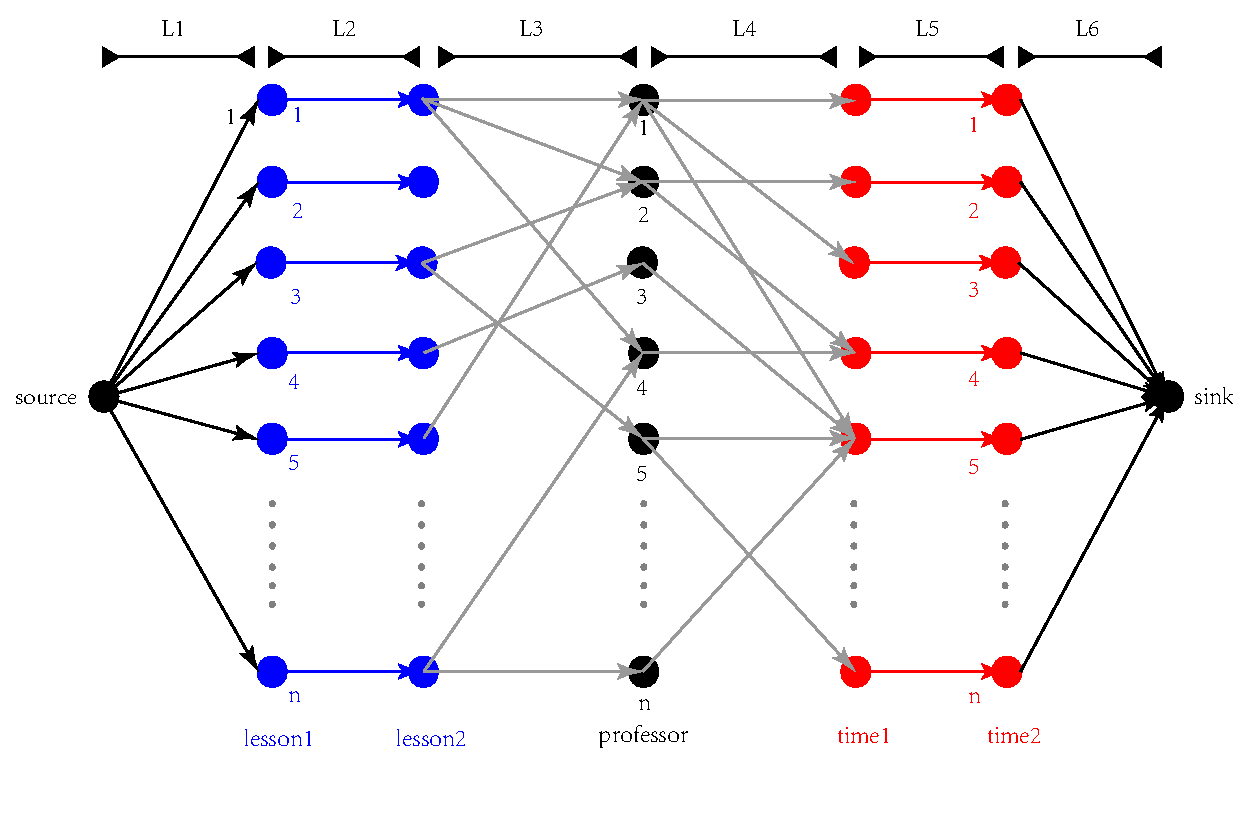
\includegraphics[width=0.8\textwidth]{pictures/1_1.pdf}
        \caption{\textbf{Model Visualization}}\label{Graph0}
        \end{figure}
\item [(2)] \textbf{Explaination:} In Figure.\ref{Graph0}, all the flow is rightward from $source$ to $sink$, all edge have capacity $1$. $L1 \rightarrow L6$ have their own meaning.
\begin{itemize}
\item \textbf{L1 and L6:} L1 have edges from source to all the lesson nodes, L2 have edges from all time nodes to sink. Then once a path from source to sink is set, a likeness matching is set as well. In short, the likeness-matching $k$ is the value of the flow-network, which means
$$k=v(f)=\sum_{e\ out\ of\ source}^{flow-network}f(e)=\sum_{e\ in\ to\ sink}^{flow-network}f(e)$$
\item \textbf{L2 and L5:} lesson1 and lesson2, time1 and time2 are repeated layers. In L2 and L5 each, it have one-to-one matching edge, which means
$$edge_{lesson1(i),lesson2(j)}\ exists,\ (i=j);\ edge_{time1(i),time2(j)}\ exists,\ (i=j)$$
We set this two layers to ensure one $time$ and $lesson$ node is selected by one professor, because each node only have capacity 1 in L2 and L5. 
\item \textbf{L3:} Every edge $e_{i,j}$ in L3 is set iff professer $j$ likes lesson $i$. Once a edge has flow 1, it means this lesson $i$ is selected by professer $j$, which means
$$edge_{lesson2(i),professor(j)}\ exists,\ (professor\ j\ likes\ lesson\ i)$$
And since L2, one lesson can't be selected twice.
\item \textbf{L4:} Every edge $e_{i,j}$ in L4 is set iff professer $i$ likes time $j$. Once a edge has flow 1, it means this time $j$ is selected by professer $i$, which means
$$edge_{professor(i),time(j)}\ exists,\ (professor\ i\ likes\ time\ j)$$
And since L5, one time can't be selected twice.
\end{itemize}
\item [(3)] \textbf{Correctness:} As we set each edge has capacity 1, it means 
$$ f(e)=\left\{
            \begin{array}{rcl}
            1       &      & {,e \in selected,}\\
            0     &      & {,e \notin selected.}
            \end{array} \right. $$
and we can define that once a path have all edges satisfy $f(e)=1$, the matching professor-lesson-time is set. Acoording to correctness of Ford-Fulkerson Algorithm, it must find the most network-flow, therefore, we just need to prove that, for all the professor, a lesson or a time-slot can be selected twice.\par
\textbf{Claim.} A lesson node can't have 2 or more flow to (more than 1) professor nodes; A time node can't receive 2 or more flow from (more than 1) professor nodes.
\par
\textbf{Proof.} We can assume lesson2 node $d$ have 2 or more flow to (more than 1) professor nodes, which means
$$\sum_{e\ out\ of\ d}^{flow-network}f(e) \geq 2$$
according to flow-network $Conservation$ property, 
$$\forall d \in V-\{s,t\}: \sum_{e\ out\ of\ d}f(e) =\sum_{e\ in\ to\ d}f(e)$$  
Therefore,
$$\sum_{e\ in\ to\ d}^{flow-network}f(e)=\sum_{e\ out\ of\ d}^{flow-network}f(e) \geq 2$$
Since lesson2 node $d$ just have a flow-in edge with capacity 1, it result in contradiction, which means a lesson node can't have 2 or more flow to (more than 1) professor nodes.\par
$(*)$ We can samely prove a time node can't receive 2 or more flow from (more than 1) professor nodes.
\item [(4)] \textbf{Operation:} We can use Ford-Fulkerson Algorithm to find the max flow in this model, as we prove the correctness above, max professor-lesson-time equals max flow, which means
$$\max[ v(f)] = \max[ matching_{professor-lesson-time}]$$
We can easily get the answer with this algorithm.
\end{itemize}
\end{solution}

\end{enumerate}

\vspace{20pt}

\textbf{Remark:} You need to include your .pdf and .tex files in your uploaded .rar or .zip file.

%========================================================================
\end{document}
